\section{Methodology}
\subsection{Simulation Procedure}
We introduce the overall simulation procedure to achieve our goal. The basic idea of the simulation is to verify and visualize the theories we use. We firstly set signal models to be used to measure waveform and signal strength. Path Loss, Gaussian distribution and Rayleigh distribution are used in this step. Secondly, we design a model of robots that has a transmitter and receivers, and simulation field where the robots are placed and our algorithm are applied. Then we apply MUSIC algorithm to estimate the DoA.


\begin{figure}[ht]
	\centering
	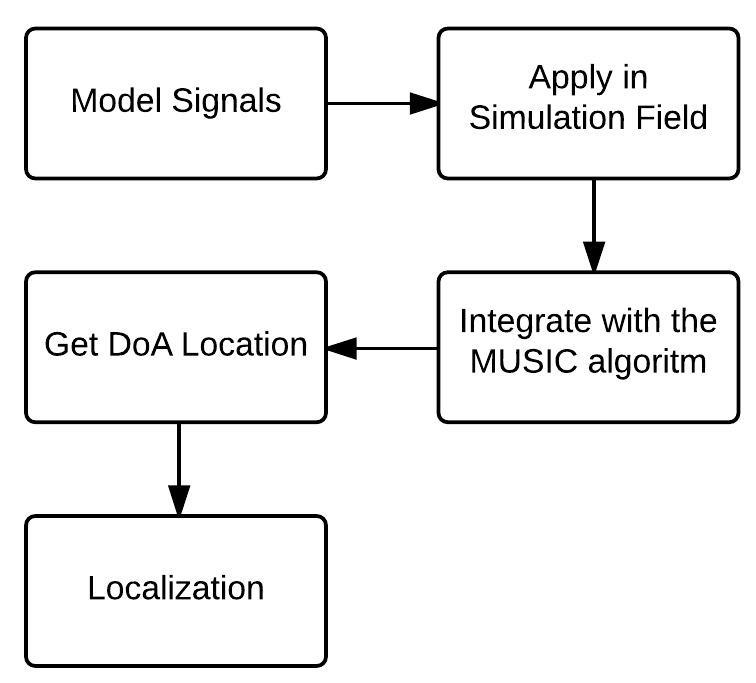
\includegraphics[width=0.4\textwidth]{procedure}
	\caption{Simulation Procedure}
	%\label{fig1}
	\end{figure}
	
In the simulation is designed to see locations of robots and estimated distance by signal strength measured by robot's receivers. The location of the robots and some ranges from the robot are marked. The simulation assumes that field is a 2-D space that ranges 1000 meters by 1000 meters. The robots consist of a transmitter and four receivers with a interval of 0.6 meters. The marked range from robots are 200 meters and 100 meters and 20 meters representing the sensory range and the communication range, the rejection range respectively.



\begin{figure}[ht]
	\centering
	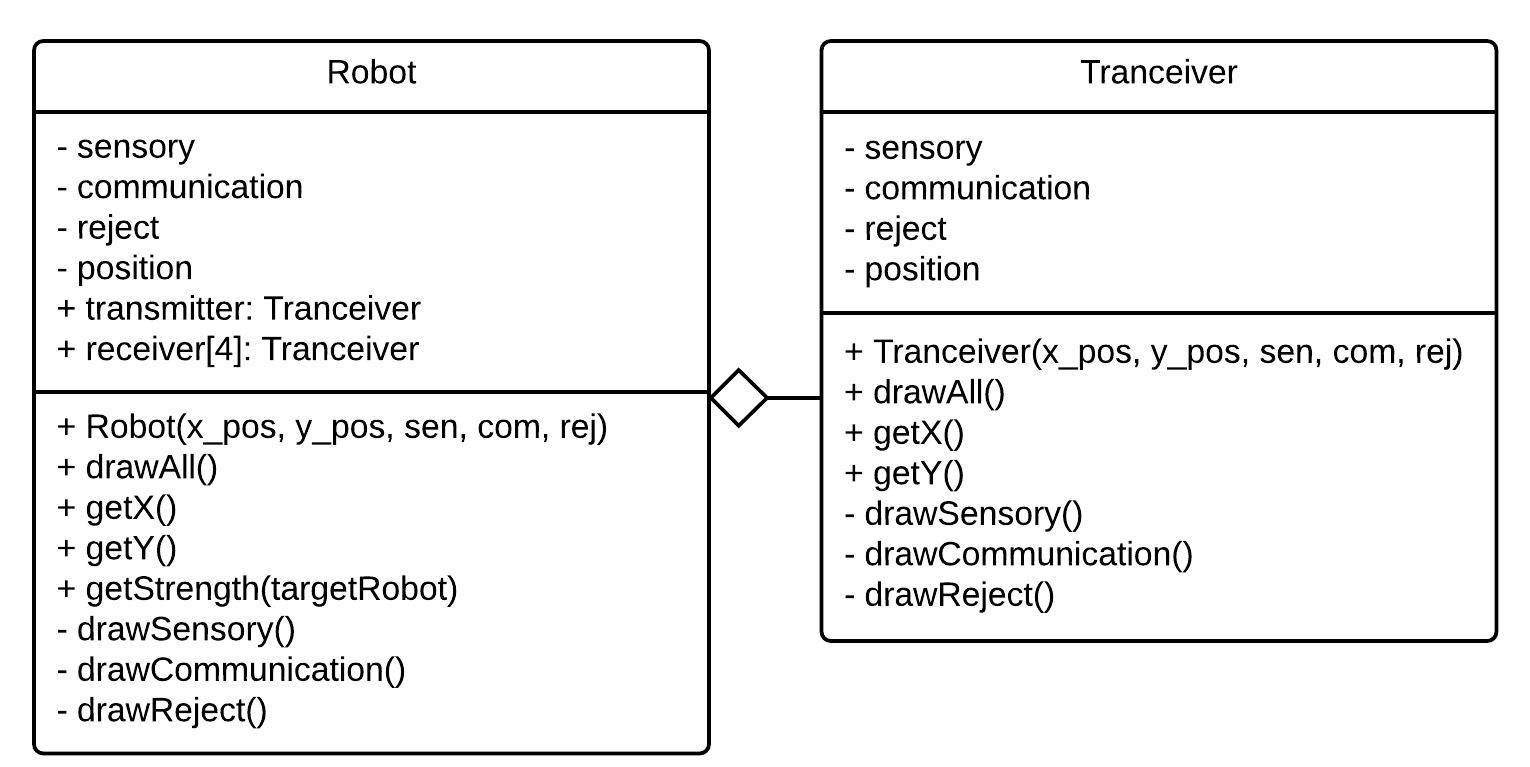
\includegraphics[width=0.4\textwidth]{classDiagram}
	\caption{Class Diagram of the simulation}
	%\label{fig1}
	\end{figure}
	

The simulation is written in MATLAB. The simulation consists of five files: 
\begin{itemize}
	\item simulation.m
	\item Robot.m
	\item Tranceiver.m
	\item simulation.m
	\item getSignalStrength.m
	\item drawCircle.m.
\end{itemize}

The drawCircle.m is used to draw circles on the simulation field to visualize the ranges of robots.

The getSignalStrength.m defines our signal model and accepts a distance value as an argument then returns a value of signal Strength. The model of signal will be discussed later.

Tranceiver.m defines the model of the signal transmitter and receiver using class. This class has four kinds of class member: sensory, communication, reject, and position. The class member sensory, communication, and reject are floating points in meters, representing those name of range. The class member position represents four 

Robot.m defines the class of the robot that has five instances of Tranceiver class:one is for transmitter and the other four is for receiver. This class has a method getStrength() that takes another instance of Robot and calculate signal strength between two robots. 

\subsection{Formula}
\begin{itemize}
\item To simplify our simulation, we decide to use a simple version of path loss, which is:
\begin{equation}
L(d)=10*n*log_{10}d + C
\end{equation}
where $L$ is the path loss in decibels, $n$ is the path loss exponent, $d$ is the distance between the transmitter and the receiver, usually measured in meters, and $C$ is a constant which accounts for system losses.
\vspace{1cm}

\item Rayleigh distributed probability density function is:
\begin{equation}
p_{R}(r)={\frac {2r}{\Omega }}e^{-r^{2}/\Omega },\ r\geq {}0
\end{equation}
where $R$ is random variable, $\Omega = E(R^{2})$.
\vspace{1cm}

\item The probability density function $p$ of a normal distribution random variable $z$ in our case is:
\begin{equation}
p_{G}(z)={\frac {1}{ {\sqrt {2\pi }}}}e^{-{\frac {z^{2}}{2}}}
\end{equation}
where $z$ represents the grey level, $\mu$  the mean value and $\sigma$  the standard deviation
\vspace{1cm}
\par
\item The frequency estimation function for MUSIC is:
\begin{equation}
\hat P_{MU}(e^{j \omega}) = \frac{1}{\sum_{i=p+1}^{M} |\mathbf{e}^{H} \mathbf{v}_i|^2},
\end{equation}
where $\mathbf{v}_i$ are the noise eigenvectors and
\begin{equation}
\mathbf{e} = \begin{bmatrix}1 & e^{j \omega} & e^{j 2 \omega} & \cdots & e^{j (M-1) \omega}\end{bmatrix}^T.
\end{equation}
\end{itemize}
%\begin{figure}[h]
%\centering
%\includegraphics[width=0.8\linewidth]{img/img1}
%\caption{3D terrain surface}
%\label{fig4}
%\end{figure} 